\documentclass[12pt]{report}

\usepackage{natbib}
\usepackage{graphicx}
\usepackage{lipsum}
\usepackage[bookmarks=false, colorlinks=true, citecolor=blue, linkcolor=blue]{hyperref}

\usepackage[a4paper,left=2.5cm,right=2.5cm,top=2.5cm,bottom=2.5cm]{geometry}
\usepackage{fancyhdr}
\usepackage{datetime}


\usepackage[listings]{tcolorbox}

\newtcblisting{commandshell}{colback=white,colupper=black,colframe=black!25, listing only}

\pagestyle{fancy}

\renewcommand{\chaptermark}[1]{\markboth{\MakeUppercase{\chaptername\ #1}}{}}

\renewcommand{\chaptername}{}

\usepackage{titlesec}
\titleformat{\chapter}[hang]{\bfseries\huge}{}{0ex}{\thechapter.~}[]
\titleformat{name=\chapter,numberless}[hang]{\bfseries\huge}{}{0ex}{}[]
\titleformat{\section}[block]{\bfseries\Large}{}{0ex}{\thesection~}[]
\titleformat{name=\section,numberless}[block]{\bfseries\Large}{}{0ex}{}[]
\titleformat{\subsection}[block]{\bfseries\large}{}{0ex}{\thesubsection~}[]
\titleformat{name=\subsection,numberless}[block]{\bfseries\large}{}{0ex}{}[]



\def\mydate{\leavevmode\hbox{\the\day~\monthname, \the\year}}
\def\twodigits#1{\ifnum#1<10 0\fi\the#1}

% Standard journal abbreviations
% Mostly as used by ADS, with a few additions for journals where MNRAS does not
% follow normal IAU style.

\newcommand\aap{A\&A}                % Astronomy and Astrophysics
\let\astap=\aap                          % alternative shortcut
\newcommand\aapr{A\&ARv}             % Astronomy and Astrophysics Review (the)
\newcommand\aaps{A\&AS}              % Astronomy and Astrophysics Supplement Series
\newcommand\actaa{Acta Astron.}      % Acta Astronomica
\newcommand\afz{Afz}                 % Astrofizika
\newcommand\aj{AJ}                   % Astronomical Journal (the)
\newcommand\ao{Appl. Opt.}           % Applied Optics
\let\applopt=\ao                         % alternative shortcut
\newcommand\aplett{Astrophys.~Lett.} % Astrophysics Letters
\newcommand\apj{ApJ}                 % Astrophysical Journal
\newcommand\apjl{ApJ}                % Astrophysical Journal, Letters
\let\apjlett=\apjl                       % alternative shortcut
\newcommand\apjs{ApJS}               % Astrophysical Journal, Supplement
\let\apjsupp=\apjs                       % alternative shortcut
% The following journal does not appear to exist! Disabled.
%\newcommand\apspr{Astrophys.~Space~Phys.~Res.} % Astrophysics Space Physics Research
\newcommand\apss{Ap\&SS}             % Astrophysics and Space Science
\newcommand\araa{ARA\&A}             % Annual Review of Astronomy and Astrophysics
\newcommand\arep{Astron. Rep.}       % Astronomy Reports
\newcommand\aspc{ASP Conf. Ser.}     % ASP Conference Series
\newcommand\azh{Azh}                 % Astronomicheskii Zhurnal
\newcommand\baas{BAAS}               % Bulletin of the American Astronomical Society
\newcommand\bac{Bull. Astron. Inst. Czechoslovakia} % Bulletin of the Astronomical Institutes of Czechoslovakia 
\newcommand\bain{Bull. Astron. Inst. Netherlands} % Bulletin Astronomical Institute of the Netherlands
\newcommand\caa{Chinese Astron. Astrophys.} % Chinese Astronomy and Astrophysics
\newcommand\cjaa{Chinese J.~Astron. Astrophys.} % Chinese Journal of Astronomy and Astrophysics
\newcommand\fcp{Fundamentals Cosmic Phys.}  % Fundamentals of Cosmic Physics
\newcommand\gca{Geochimica Cosmochimica Acta}   % Geochimica Cosmochimica Acta
\newcommand\grl{Geophys. Res. Lett.} % Geophysics Research Letters
\newcommand\iaucirc{IAU~Circ.}       % IAU Cirulars
\newcommand\icarus{Icarus}           % Icarus
\newcommand\japa{J.~Astrophys. Astron.} % Journal of Astrophysics and Astronomy
\newcommand\jcap{J.~Cosmology Astropart. Phys.} % Journal of Cosmology and Astroparticle Physics
\newcommand\jcp{J.~Chem.~Phys.}      % Journal of Chemical Physics
\newcommand\jgr{J.~Geophys.~Res.}    % Journal of Geophysics Research
\newcommand\jqsrt{J.~Quant. Spectrosc. Radiative Transfer} % Journal of Quantitiative Spectroscopy and Radiative Transfer
\newcommand\jrasc{J.~R.~Astron. Soc. Canada} % Journal of the RAS of Canada
\newcommand\memras{Mem.~RAS}         % Memoirs of the RAS
\newcommand\memsai{Mem. Soc. Astron. Italiana} % Memoire della Societa Astronomica Italiana
\newcommand\mnassa{MNASSA}           % Monthly Notes of the Astronomical Society of Southern Africa
\newcommand\mnras{MNRAS}             % Monthly Notices of the Royal Astronomical Society
\newcommand\na{New~Astron.}          % New Astronomy
\newcommand\nar{New~Astron.~Rev.}    % New Astronomy Review
\newcommand\nat{Nature}              % Nature
\newcommand\nphysa{Nuclear Phys.~A}  % Nuclear Physics A
\newcommand\pra{Phys. Rev.~A}        % Physical Review A: General Physics
\newcommand\prb{Phys. Rev.~B}        % Physical Review B: Solid State
\newcommand\prc{Phys. Rev.~C}        % Physical Review C
\newcommand\prd{Phys. Rev.~D}        % Physical Review D
\newcommand\pre{Phys. Rev.~E}        % Physical Review E
\newcommand\prl{Phys. Rev.~Lett.}    % Physical Review Letters
\newcommand\pasa{Publ. Astron. Soc. Australia}  % Publications of the Astronomical Society of Australia
\newcommand\pasp{PASP}               % Publications of the Astronomical Society of the Pacific
\newcommand\pasj{PASJ}               % Publications of the Astronomical Society of Japan
\newcommand\physrep{Phys.~Rep.}      % Physics Reports
\newcommand\physscr{Phys.~Scr.}      % Physica Scripta
\newcommand\planss{Planet. Space~Sci.} % Planetary Space Science
\newcommand\procspie{Proc.~SPIE}     % Proceedings of the Society of Photo-Optical Instrumentation Engineers
\newcommand\rmxaa{Rev. Mex. Astron. Astrofis.} % Revista Mexicana de Astronomia y Astrofisica
\newcommand\qjras{QJRAS}             % Quarterly Journal of the RAS
\newcommand\sci{Science}             % Science
\newcommand\skytel{Sky \& Telesc.}   % Sky and Telescope
\newcommand\solphys{Sol.~Phys.}      % Solar Physics
\newcommand\sovast{Soviet~Ast.}      % Soviet Astronomy (aka Astronomy Reports)
\newcommand\ssr{Space Sci. Rev.}     % Space Science Reviews
\newcommand\zap{Z.~Astrophys.}       % Zeitschrift fuer Astrophysik


\begin{document}

\begin{titlepage}

\vspace*{4cm}
\begin{center}

{\fontfamily{cmss}\selectfont
\Huge
\textbf{
HSIM Manual\\[0.5ex]
\Large
v210}
\vspace{2cm}

\large
\mydate
}
\end{center}
\vspace*{\fill}


\end{titlepage}

\tableofcontents

\vfill
\subsection*{Revision History}

\begin{table*}[h]
\label{tab:revision}
\begin{tabular}{lll}
\hline
Version & Date & Comments \\
\hline
1.0 & 2018-09-27 & HSIM v204 release \\
1.1 & --- & HSIM v210 release \\
\hline
\end{tabular}
\end{table*}


\subsection*{Authors of this document}
Miguel Pereira Santaella (University of Oxford)

\clearpage

\chapter{Quick Start Guide}

\section{Introduction and Installation}

HSIM is a dedicated pipeline for simulating observations with HARMONI on the Extremely Large Telescope. HSIM takes high spectral and spatial resolution input data cubes, encoding physical descriptions of astrophysical sources, and generates mock observed data cubes. The simulations incorporate detailed models of the sky, telescope, instrument, and detectors to produce realistic mock data \citep{Zieleniewski2015}.

HSIM is programmed in Python and the source code can be found at  \url{https://github.com/szieleniewski/HSIM}. It does not require any installation, just download from \url{????} and unzip. HSIM depends on the following Python packages to work:

\begin{itemize}
\setlength\itemsep{-0.5ex}
\item astropy 2.0.4
\item numpy 1.14.1
\item scipy 1.0.0
\item matplotlib 2.1.2
\item wxPython $>$ 3.0 
\end{itemize}

The code has been tested with the indicated package version, although more recent releases of these packages are likely to work as well.


\section{Running Simulations}

\subsection{Preparing the Input Datacube}

Before running HSIM, you will need an input model of your astronomical object stored as a datacube in a \textsc{fits} file. The recommended sizes for the spatial pixels (spaxels) are 1, 2, or 3 mas depending on the selected spaxel scale for HARMONI (see Table~\ref{tab:scale}). If your datacube has a different spaxel scale, HSIM will automatically interpolate\slash rebin the input datacube to the recommended values.

\begin{table*}[h]
\centering
\caption{Recommended input pixel size}
\label{tab:scale}
\begin{tabular}{cccc}
\hline
HARMONI & Recommended\\
Spaxel scale & input scale\\
(mas) & (mas) \\
\hline
4$\times$4   & 1 \\
10$\times$10 & 2 \\
20$\times$20 & 3 \\
30$\times$60 & 3 \\
\hline
\end{tabular}
\end{table*}

Similarly, it is recommended to oversample the spectral dimension of the input cube by a factor of 4 with respect to the nominal resolving power ($R$) of the selected grating (e.g., the spectral sampling for the K-grating $R$=7100 at 2.2$\mu$m should be 0.078\,nm). If your input cube has a different spectral sampling, HSIM will interpolate\slash rebin it. If possible, it is recommend to use input cubes with a spectral resolution a factor of 2 better than the $R$ of the selected grating.

The information on the spatial and spectral sampling of the input cube are passed through the \textsc{fits} file header to HSIM (Table~\ref{tab:fits_header} shows a summary of all the header keywords used by HSIM). In particular, the \texttt{CDELT1} and \texttt{CDELT2} header values are used to get the spatial scale, and \texttt{CDELT3} to obtain the spectral sampling. The spectral resolution of the input cube is indicated by \texttt{SPECRES} in wavelength units similar to \texttt{CDELT3}. The units of these values are those indicated by the \texttt{CUNIT1}, \texttt{CUNIT2}, and \texttt{CUNIT3} header values. Currently, for the spatial units (\texttt{CUNIT1} and \texttt{CUNIT2}), the accepted values are \texttt{mas} and \texttt{arcsec}. For the spectral units, \texttt{CUNIT3} and \texttt{SPECRES}, HSIM recognizes the following values: \texttt{angstrom}, \texttt{nanometers}, \texttt{nm}, \texttt{micron}, and \texttt{meter}. The size of the input cube is obtained from \texttt{NAXIS1}, \texttt{NAXIS2}, and \texttt{NAXIS3}.


The wavelength of each slice of the data cube are also calculated from the \textsc{fits} header using the following relation:
\begin{equation}\label{eq:lambda}
\lambda_i = \texttt{CRVAL3} + \texttt{CDELT3} \times (i - \texttt{CRPIX3})
\end{equation}

where $i$ is the slice number from 1 to $\texttt{NAXIS3}$. The wavelength range of the input cube and the selected grating should, at least, partially overlap.

Finally, the input data cube should be in surface brightness units indicated by \texttt{BUNIT}. The accepted units are the following: \texttt{erg/s/cm2/um/arcsec2}, \texttt{erg/s/cm2/A/arcsec2}, \texttt{J/s/m2/um/arcsec2}, and \texttt{J/s/m2/A/arcsec2}.


\begin{table*}[h]
\footnotesize
\centering
\caption{\textsc{fits} header keywords used by HSIM}
\label{tab:fits_header}
\begin{tabular}{lp{75mm}p{50mm}}
\hline
Keyword & Description & Accepted values \\
\hline
\multicolumn{3}{c}{Spatial information}\\
\hline
NAXIS\{1,2\} & Number of pixels along x-axis and y-axis\\
CTYPE1 & Type of the spatial x-axis & x, ra \\
CTYPE2 & Type of the spatial y-axis & y, dec \\
CDELT\{1,2\} & X and Y pixel size \\
CUNIT\{1,2\} & Units of CDELT\{1,2\} & mas, arcsec\\
\hline
\multicolumn{3}{c}{Spectral information}\\
\hline
NAXIS3 & Number of spectral pixels \\
CTYPE3 & Type of the spectral axis & wavelength \\
CDELT3 & Size of the spectral pixel \\
SPECRES & Spectral resolution in wavelength units &  \\
CRPIX3 & Reference pixel for the spectral axis (see Equation~\ref{eq:lambda}) \\
CRVAL3 & Wavelength of the reference pixel\\
CUNIT3 & Units of CDELT3, CRVAL3, and SPECRES & angstrom, nanometers, nm, \hbox{micron}, meter \\
\hline
\multicolumn{3}{c}{Flux units}\\
\hline
BUNIT & Flux units of the cube & erg/s/cm2/um/arcsec2, erg/s/cm2/A/arcsec2,
J/s/m2/um/arcsec2, J/s/m2/A/arcsec2 \\
\hline
\end{tabular}
\end{table*}


\subsection{Running HSIM}

Once the input data cube has been prepared, the next step is to run HSIM. HSIM comes with a graphical user interface (GUI) which can be used to define the input parameters of the simulations. Alternatively, the same options can be directly accessed from the command line.

\subsubsection{GUI}

The GUI provides a relatively easy way to list the available options. To launch HSIM in the GUI mode, type the following command\\

\begin{commandshell}
$ python hsim2.py
\end{commandshell}

Then, a window similar to that shown in Figure~\ref{fig:hsimgui} should appear. In that window, it is possible to select the input cube and the output directory and define all the parameters needed by HSIM to run the simulation (these parameters are explained in Section~\ref{s:list_options}). Clicking on the \texttt{Commence simulation} button will start the simulation. You can see how the simulation advances in the terminal window from where HSIM was called.

\begin{figure*}[!h]
\centering
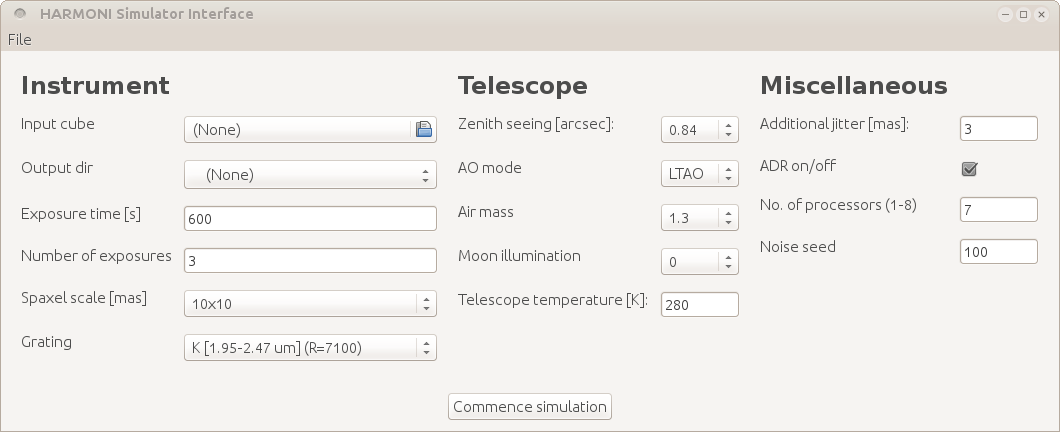
\includegraphics[width=\textwidth]{HSIM_GUI.png}
\caption{\small HSIM GUI.}\label{fig:hsimgui}
\end{figure*}

\subsubsection{Command-line}

All the GUI options can be directly accessed from the command line mode using the following command

\begin{commandshell}
$ python hsim2.py -c arg1 arg2 ...
\end{commandshell}

where \texttt{arg*} are the parameters of the simulation (see Section~\ref{s:list_options}). All the parameters are needed to run simulation. After the \texttt{-c}, you can add \texttt{-p number}, where \texttt{number} is the number of processors that will be used by HSIM. You can also add \texttt{-o directory} where \texttt{directory} is the output directory. If no output directory is specified, the default \texttt{output\_cubes} will be used and results from previous simulations might be overwritten. Finally, using \texttt{-h}, will show a short help message.


\subsection{List of Options}\label{s:list_options}

The available HSIM options are listed below. The number before them indicates the parameter order when used in the command line mode.

\begin{enumerate}
\setlength\itemsep{-0.5ex}
\item Input cube: Path of the input datacube (e.g., \texttt{datacube.fits}).
\item Exposure time: Integration time of each exposure in seconds (e.g., \texttt{600}).
\item Number of exposures (e.g., \texttt{3}).
\item Grating: Indicates the HARMONI grating. The available options are the following: \texttt{V+R, Iz+J, H+K, Iz, J, H, K, z-high, J-high, H-high, K-short, K-long}.
\item Spaxel Scale: HARMONI spatial scale in mas. The available values are the following: \texttt{4x4, 10x10, 20x20, 30+x60}.
\item Zenith seeing: Atmospheric seeing FWHM in arcsec. The available values are the following: \texttt{0.43, 0.57, 0.64, 0.72, 1.04}.
\item Air mass: Average air mass during the HARMONI observation. The available values are the following: \texttt{1.1, 1.3, 1.5, 2.0}, which correspond to zenith angles of 25$^{\circ}$, 40$^{\circ}$, 48$^{\circ}$, and 60$^{\circ}$, respectively.
\item Moon illumination: Fraction of the Moon that is illuminated at the time of the observation. A 30$^{\circ}$ separation between target and Moon is assumed. The available values are the following: \texttt{0, 0.5, 1.0}.
\item Jitter: Additional telescope PSF blur in mas. Default value is \texttt{3}.
\item Telescope temperature: Temperature of the site\slash telescope in K. This is used to calculate the telescope and part of the instrument background emission. Default value is \texttt{280}.
\item ADR on/off: Indicates if the atmospheric differential refraction is simulated. When simulated, the differential refraction is corrected in the output cubes in a way similar to what is expected from the pipieline. Available values are \texttt{True, False}.
\item Noise seed: Seed used for the random number generator during the simulation. It only affects the observed outputs (see Section~\ref{s:output}).
\item AO mode: Adaptive optics mode of the observations. The available values are the following: \texttt{LTAO, SCAO, noAO}. \texttt{LTAO} corresponds to the Laser Tomography Adaptive Optics mode,  \texttt{SCAO} to the Single Conjugate Adaptive Optics mode and \texttt{noAO} indicates that no adaptive optics corrections are applied.
% \item Detector systematics: Indicates if the detector systematics (i.e., ..) are simulated. It only affects the observed outputs (see Section~\ref{s:output}). Available values are \texttt{True, False}.
\end{enumerate}

\subsection{Output Files}\label{s:output}

HSIM stores the results of the simulation in the specified output directory (the default output directory is \texttt{output\_cubes}). The name of the output files begins with the name of the input data cube and it is followed by a suffix indicating the content of the file. The input parameters of the simulation are stored in the header of the \textsc{fits} files and also in the log file.

\begin{enumerate}
\setlength\itemsep{-0.5ex}
\item \texttt{\_noiseless\_obj\_plus\_back.fits}. Data cube containing the expected number of electrons per pixel detected by HARMONI due to the target and the background (sky, telescope, and instrument) emissions. \textbf{Cross-talk is not applied to the noiseless outputs. Therefore, their LSF is slightly narrower than that of the observed and reduced outputs.}
\item \texttt{\_noiseless\_obj.fits}. Expected number of electrons per pixel solely due to the target.
\item \texttt{\_noiseless\_back.fits}. Expected number of electrons per pixel from the background sources (sky, telescope, and instrument).
\item \texttt{\_observed\_obj\_plus\_back.fits}. Simulated observed data cube taking into account the photon noise, read noise, dark current, and cross-talk.
\item \texttt{\_observed\_back.fits}. Simulated observed sky background taking into account the photon noise, read noise, dark current, and cross-talk.
\item \texttt{\_reduced.fits}. Simulated reduced data cube created by subtracting a simulated sky observation  to the \texttt{\_observed\_obj\_plus\_back.fits} data cube.
\item \texttt{\_reduced\_SNR.fits}. Signal to noise ratio of the reduced data cube per pixel.
\item \texttt{\_std.fits}. Noise standard deviation. Includes object and sky noise (Poisson) and dark current and read noise (Gaussian).
\item \texttt{\_PSF.fits}. Point spread function at the mean wavelength of the input data cube. The PSF is oversampled by a factor of 4 to 10 with respect to the other output \textsc{fits} data cubes.
\item \texttt{\_total\_em.pdf}. Plot of the background emission broken up into the individual modeled components. The average HARMONI to telescope$+$sky background ratio is indicated.
\item \texttt{\_total\_tr.pdf}. Plot of system transmission broken up into the individual modeled components.
\item \texttt{\_total\_tr.txt}. Total transmission stored as a text file.
\item \texttt{.log}. Detailed log of the simulation. The last line of this file shows if any problem was found during the simulation.
\end{enumerate}


% \clearpage
% 
% \chapter{Simulation Details}
% 
% \section{Modules}
% 
% \subsection{Sky}
% 
% \subsection{Telescope}
% 
% \subsection{Instrument}
% 
% \subsection{Detector}
% 
% \section{Simulating the Observations: Target and Sky Frames}



\cleardoublepage
\phantomsection

\addcontentsline{toc}{chapter}{Bibliography}

\bibliographystyle{mnras.bst}
\bibliography{biblio}


\end{document}
